\documentclass[tikz, border=15pt]{standalone}
\usetikzlibrary{shapes, arrows.meta, positioning, calc}

\begin{document}
	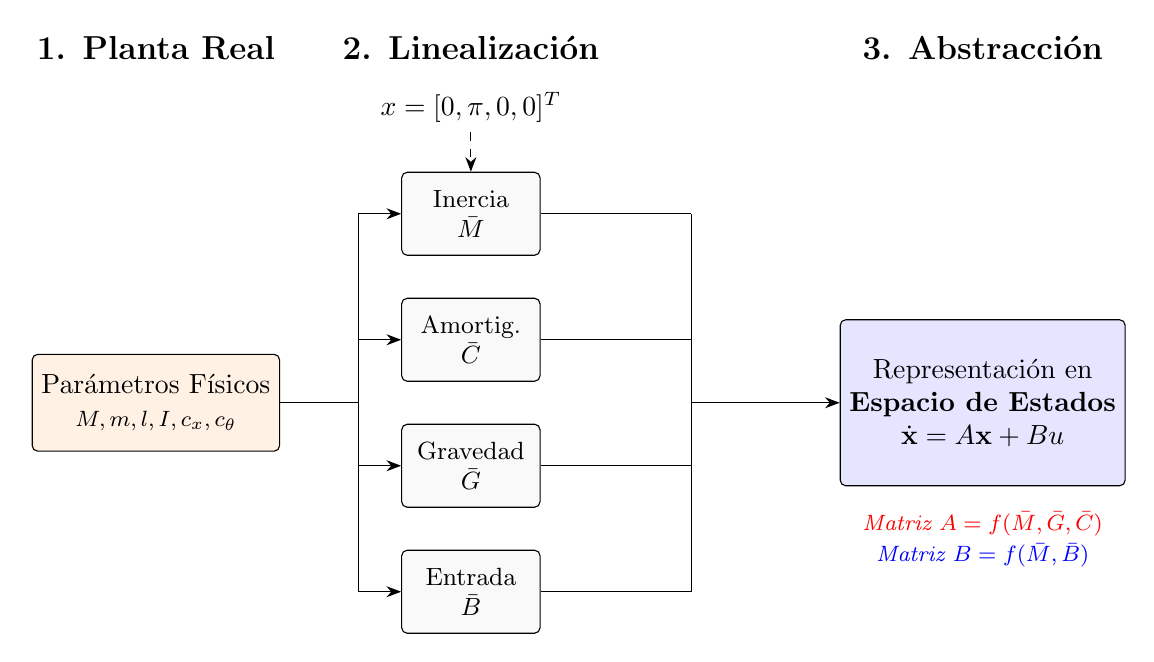
\begin{tikzpicture}[
		block/.style = {draw, rectangle, minimum height=3.5em, minimum width=7em, align=center, rounded corners=2pt},
		% Estilo para las matrices de robótica
		matrix_block/.style = {draw, fill=gray!5, rectangle, minimum height=3em, minimum width=5em, align=center, rounded corners=2pt, font=\small},
		>={Stealth[scale=1.1]}
		]
		
		% --- ENTRADA: PARÁMETROS FÍSICOS ---
		\node [block, fill=orange!10] (params) at (0,0) {Parámetros Físicos \\ \footnotesize $M, m, l, I, c_x, c_\theta$};
		
		% --- NIVEL 1: MATRICES DINÁMICAS (Robótica) ---
		\node [matrix_block] (M)     at (4,  2.4) {Inercia \\ $\bar{M}$};
		\node [matrix_block] (C)     at (4,  0.8) {Amortig. \\ $\bar{C}$};
		\node [matrix_block] (G)     at (4, -0.8) {Gravedad \\ $\bar{G}$};
		\node [matrix_block] (B_mat) at (4, -2.4) {Entrada \\ $\bar{B}$};
		
		% Punto de equilibrio alimentando a la linealización
		\node [above=0.5cm of M] (eq_point) {$x = [0, \pi, 0, 0]^T$};
		
		% --- NIVEL 2: ESPACIO DE ESTADOS ---
		% Desplazado a X=10.5 para dar más espacio a la flecha
		\node [block, fill=blue!10, minimum height=6em, minimum width=10em] (ss) at (10.5, 0) {
			Representación en \\ \textbf{Espacio de Estados} \\
			$\dot{\mathbf{x}} = A\mathbf{x} + Bu$
		};
		
		% --- CONEXIONES ---
		% De parámetros a matrices
		\draw [->] (params.east) -- ++(1,0) |- (M.west);
		\draw [->] (params.east) -- ++(1,0) |- (C.west);
		\draw [->] (params.east) -- ++(1,0) |- (G.west);
		\draw [->] (params.east) -- ++(1,0) |- (B_mat.west);
		
		% Punto de equilibrio a la inercia
		\draw [dashed, ->] (eq_point) -- (M.north);
		
		% --- CONVERGENCIA HACIA ESPACIO DE ESTADOS ---
		% 1. Líneas horizontales sin flecha hasta la coordenada X = 6.8
		\draw [-] (M.east) -- (6.8, 2.4);
		\draw [-] (C.east) -- (6.8, 0.8);
		\draw [-] (G.east) -- (6.8, -0.8);
		\draw [-] (B_mat.east) -- (6.8, -2.4);
		
		% 2. Línea vertical que une todas las salidas
		\draw [-] (6.8, 2.4) -- (6.8, -2.4);
		
		% 3. Única flecha recta desde el centro de la línea vertical hasta el bloque final
		\draw [->] (6.8, 0) -- (ss.west);
		
		% --- ANOTACIONES DE LAS SUBMATRICES ---
		\node [below=0.2cm of ss, font=\footnotesize\itshape, text=red] {Matriz $A = f(\bar{M}, \bar{G}, \bar{C})$};
		\node [below=0.6cm of ss, font=\footnotesize\itshape, text=blue] {Matriz $B = f(\bar{M}, \bar{B})$};
		
		% --- TÍTULOS DE LAS ETAPAS ---
		\coordinate (title_y) at (0, 4.5);
		\node [font=\bfseries\large] at (params |- title_y) {1. Planta Real};
		\node [font=\bfseries\large] at (M |- title_y)      {2. Linealización};
		\node [font=\bfseries\large] at (ss |- title_y)     {3. Abstracción};
		
	\end{tikzpicture}
\end{document}